\section{The handle construction}\label{sec:shd}

The construction is an explicit version of the surface packing lemma of \cite[\S3.2]{OpenAI2026}. For the
higher-dimensional model inputs of \Mref{Definition}{def:mech-model} the choices are fixed in \S\ref{sec:native-toric};
this section supplies the finite primitive used there, the handle data of the diagonal-quadric presentation, and the
nondegeneracy and flow statements behind \Msec{sec:hdl}. The periodic four-dimensional instance is treated in
\S\ref{sec:shd-four}. Several objects of \S\S\ref{sec:shd-primitive}--\ref{sec:shd-proof} (the bump forms, the tree primitives and the
normalisation) are constructed in \S\ref{sec:native-toric}, which comes after \S\ref{sec:str} because it also fixes the
Moser fields and the maps $\psi_i$; \S\ref{sec:shd-four} does not use \S\ref{sec:native-toric}.

\subsection{The finite primitive}\label{sec:shd-primitive}

\begin{construction}[Coordinate primitive]\label{cons:shd-primitive}
\lean{SymplecticPacking.HighDim.ToricPackingStages.RawAmbientBox.formPrimitive,
SymplecticPacking.HighDim.ToricPackingStages.RawSurfacePresentation.primitiveOperator}
Let $r\,dx\wedge dy$ be a smooth two-form with compact support in an open coordinate rectangle $I\times I'$, put
$M(x)=\int r(x,y)\,dy$ and fix a smooth bump $b$ with compact support in $I'$ and $\int b=1$. With integrals starting
at the lower endpoints of $I$ and $I'$, put
\begin{equation}\label{eq:shd-Ploc}
 P(r)=-\left[\int^y\bigl(r(x,t)-b(t)M(x)\bigr)\,dt\right]dx
       +b(y)\left[\int^xM(t)\,dt\right]dy .
\end{equation}
For a finite presentation (Definition~\ref{def:shd-presentation}) with partition weights $\zeta_i$, unit-mass bumps
$\eta_i$ and tree primitives $T_i$ (\S\ref{sec:native-toric}), the operator is
\begin{equation}\label{eq:shd-PSigma}
 \mathcal P\omega=\sum_i\left[P_i(\zeta_i\omega-m_i(\omega)\eta_i)+m_i(\omega)T_i\right],\qquad m_i(\omega)=\int\zeta_i\omega .
\end{equation}
Each local coefficient is extended by zero only after multiplication by its compactly supported weight.
\end{construction}

\begin{lemma}[Primitive identity]\label{lem:shd-primitive}
\lean{SymplecticPacking.HighDim.ToricPackingStages.RawSurfacePresentation.primitiveOperator_data,
SymplecticPacking.HighDim.ToricPackingStages.RawSurfacePresentation.primitiveOperator_family_smooth}
If $\int_{I\times I'}r\,dx\wedge dy=0$, then $P(r)$ has compact support in $I\times I'$ and $dP(r)=r\,dx\wedge dy$. Let
$\omega(p)$ be a smooth family of two-forms supported in the correction core with $m(\omega(p))=\sum_im_i(\omega(p))=0$.
Then $d_\Sigma\mathcal P\omega(p)=\omega(p)$, and $\mathcal P\omega(p)$ has fixed compact support in the interior of the
model base and depends smoothly on $(p,x)$.
\end{lemma}
\begin{proof}
The differential of the first term of \eqref{eq:shd-Ploc} is $(r-bM)\,dx\wedge dy$, that of the second is
$bM\,dx\wedge dy$. The $dx$-coefficient vanishes for $y$ below $\operatorname{supp}r\cup\operatorname{supp}b$, and above it
because $\int(r(x,t)-b(t)M(x))\,dt=0$; it vanishes for $x$ outside the $x$-projection of $\operatorname{supp}r$. The
$dy$-coefficient vanishes outside $\operatorname{supp}b$ in $y$, below $\operatorname{supp}M$ in $x$, and above it because
$\int M=0$. For the operator, every argument of $P_i$ has zero mass, so $dP_i(\cdot)$ returns it; the tree primitives
satisfy $dT_i=\eta_i-\eta_0$ (\S\ref{sec:native-toric}); hence
$d\mathcal P\omega=\omega-m(\omega)\eta_0=\omega$. All integrals are over fixed compact coordinate domains with smooth
integrands, which gives the support and smoothness statements.
\end{proof}

\subsection{The handle data of the diagonal quadric}\label{sec:shd-handle-data}

\begin{definition}[Finite presentation]\label{def:shd-presentation}
\lean{SymplecticPacking.HighDim.ToricPackingStages.RawSurfacePresentation,
SymplecticPacking.HighDim.ToricPackingStages.quadricModelRawPresentation}
A finite presentation consists of coordinate maps with explicit inverses, compact inner and outer coordinate boxes,
partition weights $\zeta_i$ ($\zeta_i$ supported in outer box $i$, $\sum_i\zeta_i=1$ on the union of the inner boxes),
unit-mass bumps in the boxes and in the overlaps of parent and child, and a rooted tree on the boxes in which every
box $i\ne0$ has a parent $j<i$ whose overlap with box $i$ contains a coordinate box.
\end{definition}

\begin{construction}[Handle and normalisation data]\label{cons:shd-handle-data}
\lean{SymplecticPacking.HighDim.ToricPackingStages.QuadricRawDual.actualDual,
SymplecticPacking.HighDim.ToricPackingStages.quadricModelRawPresentation}
For the diagonal affine curve $\Sigma$ of Definition~\ref{def:qdr-curve} take the transverse cylinder
$e(s,\theta)$, the dual form $\beta=\beta_0-d(e_*(\chi F))$ and the clock profile $b$ of Proposition~\ref{prop:vtr-handle}.
The annular coordinate of \Mref{Definition}{def:hdl-handle-data}(a) is $s_{\rm a}=s$ on $|s|<w=\frac18$, with working
half-width $b=\frac1{16}$; on $|s|<\frac5{32}$, which contains this annulus, $e^*\beta=b(\theta)\,d\theta$. The reference
primitive is $\Gamma_{\rm ref}=\lambda=d^c\log(1+|z|^2)$, with $\Lambda=\sigma$, and $\Gamma_{\rm phys}(p)=(1-2|p|)\lambda$,
so $\kappa(p)=(1-2|p|)\sigma$. On $\Sigma_\ell$ with $R_\ell\ge5$ the correction atlas is the family of
Lemma~\ref{lem:vtr-cells} with $R=R_\ell-1$, and the flow atlas is the same family with $R=R_\ell$, restricted to a
neighbourhood of $\Sigma_\ell$. The collar cutoff is
$\chi_\partial=S\bigl((|t|^2-(R_\ell-2)^2)/((R_\ell-1)^2-(R_\ell-2)^2)\bigr)$. The mixed model of \S\ref{sec:two-mixed} uses
the same base data, and the six-dimensional model uses them with its physical primitive $\Gamma(p)$ of
Definition~\ref{def:sxm-data}.
\end{construction}

\begin{lemma}[Handle certificates]\label{lem:shd-handle-data}
\lean{SymplecticPacking.HighDim.ToricPackingStages.QuadricRawDual.actualDual_contMDiff,
SymplecticPacking.HighDim.ToricPackingStages.quadricRawHandle_dual, SymplecticPacking.BranchSmall.QHandle.dual_closed,
SymplecticPacking.HighDim.ToricPackingStages.quadricRawHandle_dual, SymplecticPacking.BranchSmall.QHandle.dual_compact}
The form $\beta$ is smooth, closed and supported in $\{|t|\le3\}\subset\operatorname{int}\Sigma_\ell$; on the annulus it equals
$b(\theta)\,d\theta$ with $b\ge0$, $b>0$ on $(\frac14,\frac34)$ and $\int_0^1b=1$. The inner boxes of the correction atlas
cover $\{|t|\le R_\ell-1\}$, which contains the support of $1-\chi_\partial$ and the handle, and all its outer boxes lie in
$\operatorname{int}\Sigma_\ell$. For $p\in\Delta_h$, $\kappa(p)\ge(1-2h)\Lambda$ on all of $\Sigma_\ell$, so the correction region
of \Mref{Definition}{def:hdl-handle-data}(d) is $\Sigma_\ell$ with $\kappa_-=1-2h$. The inner boxes of the flow atlas cover
$\Sigma_\ell$.
\end{lemma}
\begin{proof}
The statements on $\beta$ and $b$ are Proposition~\ref{prop:vtr-handle}; the annuli $A$, $C$ lie in $|t|\le\frac53$
(proof of Lemma~\ref{lem:vtr-tail}). The covering and containment statements are Lemma~\ref{lem:vtr-cells} with
$R=R_\ell-1$ and $R=R_\ell$: its branch-square condition $i+\frac1{16}<(R+1)^2$ holds because $i\le m<R_\ell-1$. The
cutoff $\chi_\partial$ vanishes for $|t|\le R_\ell-2$, so $\operatorname{supp}(1-\chi_\partial)\subset\{|t|\le R_\ell-1\}$, and the
handle lies in $|t|\le3<R_\ell-1$. Finally $1-2|p|\ge1-2h>0$ on $\Delta_h$.
\end{proof}

\subsection{Normalisation and the budget}\label{sec:shd-datum}

\begin{lemma}[Normalised datum]\label{lem:shd-datum}
\lean{SymplecticPacking.HighDim.RawNormalizationSpec,
SymplecticPacking.HighDim.RawModelAgreement.normalization_target}
Let $\gamma_*$ be the reserve of the comparison datum. The primitive $\Gamma_n$ of
Construction~\ref{cons:native-normalization} agrees with $\Gamma_{\rm phys}$ near $\partial\Sigma_\ell$, its base curvature
$d_\Sigma\Gamma_n(p)=\kappa_{\rm sm}(p)+H^*(p)\eta$ is positive for $p\in\Delta$, and on the annulus
\begin{equation}\label{eq:shd-Gamma}
 \Gamma_n(p)=e_\Lambda\Gamma_{\rm ref}+f(s)H^*(p)\beta .
\end{equation}
The mass $H^*$ is smooth, nonnegative on $\Delta$, and $H^*\ge\Hb-\gamma_*/16$.
\end{lemma}
\begin{proof}
This is Proposition~\ref{prop:native-normalization}. Agreement near the boundary holds because the corrections
$\mathcal P(\cdot)$, $c_p\beta$ and $d_\Sigma(\zeta u_p)$ are supported in the correction core, in $\operatorname{supp}\beta$ and in the
annulus, all compact in $\operatorname{int}\Sigma_\ell$ (Lemma~\ref{lem:shd-handle-data}).
\end{proof}

For given capacities $\rho_i<a_i$ the layers use
\begin{equation}\label{eq:shd-constants}
 \rho_i^\sharp=\frac{3a_i+\rho_i}{4},\qquad
 \varepsilon_i=\frac{a_i-\rho_i^\sharp}{4}.
\end{equation}
The model estimates are
\begin{equation}\label{eq:shd-collar}
 \int_{\Sigma_\ell}\chi_\partial\kappa(p)\le\gamma_*/32,\qquad
 e_\Lambda\int_{\Sigma_\ell}\Lambda\le\gamma_*/32\qquad(p\in\Delta),
\end{equation}
and with
\begin{equation}\label{eq:shd-ksm}
 \kappa_{\rm sm}=\chi_\partial\kappa+(1-\chi_\partial)e_\Lambda\Lambda,
 \qquad H^*=\Hb-\int_{\Sigma_\ell}\kappa_{\rm sm}
\end{equation}
they give, for $w\in V_\Delta$, by \Mref{Proposition}{prop:hdl-layers}(ii),
\begin{multline}\label{eq:shd-budget}
 H^*\ge\Hb-\gamma_*/16,\\
 R^*(w)=K(p(q^{-1}w))-K(p(w))+H^*(p(w))-\sum_ih_i(p(w))\ge\gamma-\gamma_*/16>0 .
\end{multline}

\begin{lemma}[Nondegeneracy and the Gram cutoffs]\label{lem:shd-nbhd}
\lean{SymplecticPacking.HighDim.RawFlowAtlasSpec.pathCutoff_spec}
Let $K=V_\Delta(E)$. For $j=0,1,2$ and $t\in[0,1]$ the forms $\Omega_{j,t}$ of \S\ref{sec:native-toric} are symplectic at every
point of $K$, hence on an open neighbourhood of $[0,1]\times K$ in $[0,1]\times E$. The cutoff $\chi_j$ of
\S\ref{sec:native-toric} equals one on a neighbourhood of $[0,1]\times K$, and $\chi_j(t,\cdot)$ has compact support contained in
the set where $\Omega_{j,t}$ is nondegenerate.
\end{lemma}
\begin{proof}
All three paths are closed, being exact. By \Mref{Lemma}{lem:hdl-top-power}(a), for a toric primitive $Q$ the top power of
$\omega_V+dQ$ is $n\,\omega_V^m\wedge d_\Sigma Q$; mixed terms $dp_j\wedge(\cdot)$ do not contribute.

\emph{Path $0$.} $d_\Sigma Q_{0,t}=(1-t)\kappa(p)+t(\kappa_{\rm sm}(p)+H^*\eta)$. For $p\in\Delta$, $\kappa(p)>0$
(\Mref{Definition}{def:mech-model}), $\kappa_{\rm sm}(p)$ is a convex combination of $\kappa(p)$ and $e_\Lambda\Lambda>0$, and
$H^*\eta\ge0$ since $H^*\ge0$ and $\eta=f'b\,ds\wedge dv\ge0$. So the base form is positive.

\emph{Path $1$.} Off $E|_{\mathcal A}$, $\Omega_{1,t}=\Omega_{0,1}$. On $E|_{\mathcal A}$, $\Omega_{1,t}=\mathcal D_t^*(\omega_V+e_\Lambda\Lambda+d(G_t\beta))$
(\Mref{Lemma}{lem:hdl-suspension}(ii)), whose top power at $\mathcal D_t(x)$ is, by \Mref{Lemma}{lem:hdl-top-power}(b),
$n(e_\Lambda a_\Lambda+b\,f'(s)H^*(p(q_t^{-1}w')))\,\omega_V^m\wedge ds\wedge dv$ with $w'$ the fibre point of $\mathcal D_t(x)$.
Since $q_\tau(V_\Delta)=V_\Delta$ for all $\tau$ (\Mref{Definition}{def:mech-datum}), $x\in K$ gives $w'\in V_\Delta$ and
$q_t^{-1}w'\in V_\Delta$, so $H^*\ge0$ there; $e_\Lambda a_\Lambda>0$, $b\ge0$, $f'\ge0$, and $\mathcal D_t$ is a diffeomorphism.

\emph{Path $2$.} On $E|_{\mathcal A}$, $\Omega_{2,t}=\mathcal D^*(\omega_V+e_\Lambda\Lambda+d(\hat G_t\beta))$ by (\Mnum{eq:hdl-final}),
with top-power coefficient $e_\Lambda a_\Lambda+b\,\partial_s\hat G_t$ at $\mathcal D(x)$; here
$\partial_s\hat G_t=(1-t)f'H^*(p(q^{-1}w'))+t\,\partial_sG_{\rm f}\ge0$ on $\mathcal A\times V_\Delta$ by the previous case and
\Mref{Proposition}{prop:hdl-layers}(iii). Off $E|_{\mathcal A}$, $\Omega_{2,t}=\Omega_{0,1}+t\,dJ\wedge\beta$ differs from
$\Omega_{0,1}$ by a mixed term and has the same top power.

Thus each $\Omega_{j,t}^n\ne0$ on the compact set $[0,1]\times K$; since nondegeneracy is an open condition and the forms
depend smoothly on $(t,x)$, it holds on an open neighbourhood. For the cutoff, at each point of $K$ some flow-atlas
bump $w_i$ equals one and the determinant of $\Omega_{j,t}$ in chart $i$ is nonzero, so $g_j>0$ on $[0,1]\times K$ and
$\mu_j>0$. The factor $S(4g_j/\mu_j-1)$ equals one where $g_j\ge\mu_j/2$, and $S(2(R+1-|w|^2))$ equals one where
$|w|^2\le R+\frac12$; both sets contain an open neighbourhood of $[0,1]\times K$. Conversely $\chi_j(t,z)\ne0$ forces
$g_j(t,z)>\mu_j/4>0$, so some $w_i(z)\ne0$ with nonzero determinant in chart $i$, and $|w|^2<R+1$; the set
$\{g_j(t,\cdot)\ge\mu_j/4,\ |w|^2\le R+1\}$ is closed, its base projection lies in the compact union of the supports of the $w_i$,
and it is therefore compact.
\end{proof}

\subsection{The three paths}\label{sec:shd-first}

\begin{proposition}[First path]\label{prop:shd-first-path}
\lean{SymplecticPacking.HighDim.RawModelAgreement.relativePath_semantic,
SymplecticPacking.HighDim.RawModelAgreement.normalization_target}
The path $\Omega_{0,t}=\omega_V+d((1-t)\Gamma_{\rm phys}+t\Gamma_n)$ has the curvature, positivity and annular endpoint
stated in \Mref{Proposition}{prop:hdl-first-path}. Its variation primitive is
\begin{equation}\label{eq:shd-alpha1}\alpha_1=\Gamma_n-\Gamma_{\rm phys},\end{equation}
which is supported in the union of the correction core, $\operatorname{supp}\beta$ and the annulus.
\end{proposition}
\begin{proof}
The base curvature and positivity are Path $0$ of Lemma~\ref{lem:shd-nbhd}; the endpoint is \eqref{eq:shd-Gamma}; the support
statement is the proof of Lemma~\ref{lem:shd-datum}.
\end{proof}

\subsection{The suspension path}\label{sec:shd-second}
\begin{proposition}[Second path]\label{prop:shd-second-path}
\lean{SymplecticPacking.HighDim.RawModelAgreement.firstPath_semantic}
The path $\Omega_{1,t}=\omega_V+d(\Gamma_n+\eta_t)$, with $\eta_t$ the suspension primitive of \Mref{Lemma}{lem:hdl-suspension},
is closed, equals $\Omega_{0,1}$ at $t=0$, and is symplectic on a neighbourhood of $V_\Delta(E)$. Over $\mathcal A$ it is the
pullback by $\mathcal D_t$ of $\omega_V+e_\Lambda\Lambda+d(G_t\beta)$, $G_t=f(s)H^*(p(q_t^{-1}w))$.
\end{proposition}
\begin{proof}
The pullback identity is \Mref{Lemma}{lem:hdl-suspension}(ii). The coefficient correction and the suspension term,
\[
 f(s)\bigl[H^*(p(q_t^{-1}q_{tf(s)}w))-H^*(p(w))\bigr]\qquad\text{and}\qquad(Q^t_s\circ q_{tf(s)})\,ds,
\]
vanish for $s\le0$ and $s\ge1$ (\Mref{Lemma}{lem:hdl-suspension}(iii)), so extension by zero is smooth and $\eta_0=0$. Nondegeneracy is Path $1$ of
Lemma~\ref{lem:shd-nbhd}.
\end{proof}

\subsection{The layer path}\label{sec:shd-layer}
\begin{proposition}[Third path]\label{prop:shd-layer-path}
\lean{SymplecticPacking.HighDim.RawModelAgreement.secondPath_semantic,
SymplecticPacking.HighDim.ToricPackingStages.native_surfaceRemainder_nonneg}
The path $\Omega_{2,t}=\omega_V+d(\Gamma_n+\eta_1+t\xi)$ is closed and symplectic on a neighbourhood of $V_\Delta(E)$. Over the
annulus it is the pullback by $\mathcal D$ of the interpolation from $G_1=fH^*\circ p\circ q^{-1}$ to
\begin{equation}\label{eq:shd-Gf}
 G_{\rm f}=J\circ p+\sum_i\varsigma_i h_i\circ p+\varsigma_*R^*,\qquad J=K-H^*,
\end{equation}
whose $s$-derivative is nonnegative on $\mathcal A\times V_\Delta$. On ball layer $i$ only the toric coefficient
$A_i(p)+\varsigma_i(s)h_i(p)$ remains. Off the annulus the correction is the toric form $J(p)\beta$.
\end{proposition}
\begin{proof}
The clocks have disjoint ordered transition intervals, and $h_i\ge0$, $R^*>0$ on $V_\Delta$ by \eqref{eq:shd-budget}; this gives
\Mref{Proposition}{prop:hdl-layers}(iii). On both end collars of $\mathcal A$ the annular correction equals $J(p)\beta$, so
$\xi$ is smooth (\Mnum{eq:hdl-xi}). Nondegeneracy is Path $2$ of Lemma~\ref{lem:shd-nbhd}.
\end{proof}

\subsection{Moser endpoints}\label{sec:shd-moser}
\begin{proposition}[The Moser maps]\label{prop:shd-moser}
\lean{SymplecticPacking.HighDim.RawFlowAtlasSpec.inverse_pathFlow_eq,
SymplecticPacking.HighDim.ToricPackingStages.RawSurfacePresentation.fullMoserFlow_spec,
SymplecticPacking.HighDim.ToricPackingStages.RawSurfacePresentation.fullMoserFlow_diffeomorph}
For $j=0,1,2$ the cut field $Y_j$, defined by $\iota_{Y_{j,t}}\Omega_{j,t}=-\chi_j\,\partial_tQ_{j,t}$ on the nondegenerate locus
and by zero elsewhere, is smooth on $[0,1]\times E$ with compact spatial support. Its time-one map $\Phi_j$ is a diffeomorphism
of $E$ with inverse the backward flow, $\Phi_j^{\pm1}(K)=K$, $\Phi_j^{\pm1}(\operatorname{int}K)=\operatorname{int}K$, and
$\Phi_j^*\Omega_{j,1}=\Omega_{j,0}$ on $K$. These are the identities of \Mref{Proposition}{prop:hdl-faces}.
\end{proposition}
\begin{proof}
By Lemma~\ref{lem:shd-nbhd}, $\chi_j(t,\cdot)$ is supported in a compact subset of the nondegenerate locus, where the
defining equation has the smooth solution $-\Omega_{j,t}^{-1}(\chi_j\partial_tQ_{j,t})$ (Cramer's rule in each chart);
this solution vanishes near the boundary of the support, so the extension by zero is smooth. A smooth field with
compact spatial support on $[0,1]\times E$ has a complete flow, and its time-one map is a diffeomorphism whose inverse is the
backward flow.

On a neighbourhood $U$ of $[0,1]\times K$ we have $\chi_j=1$, so $Y_j$ is there the Moser field of the pair
$(\Omega_{j,t},\partial_tQ_{j,t})$, which satisfies $\partial_t\Omega_{j,t}=d\,\partial_tQ_{j,t}$. Lemma~\ref{lem:native-collar} shows
that every integral curve of $Y_j$ on a subinterval of $[0,1]$ which meets $K$ (resp.\ $\operatorname{int}K$) stays in $K$
(resp.\ $\operatorname{int}K$): near $\partial\Sigma_\ell$ the variation primitives vanish, so $Y_j=0$ there; and near each outer
face $\{\mu_\nu=\ell_\nu\}$ the face moment satisfies $\iota_{X_\nu}\Omega_{j,t}=-d\mu_\nu$ and $\partial_tQ_{j,t}(X_\nu)=0$, so
$d\mu_\nu(Y_{j,t})=0$ by Lemma~\ref{lem:pre-moser}(d). The same holds in reverse time. Lemma~\ref{lem:pre-moser}(e) applied to
$\mathcal K=K$ then gives $\Phi_j(K)=K$ and $\Phi_j^*\Omega_{j,1}=\Omega_{j,0}$ on $K$; applied to the backward flow it gives
$\Phi_j^{-1}(K)=K$, and the statement for $\operatorname{int}K$ follows in the same way, since every integral curve through a
point of $\operatorname{int}K$ stays in it.
\end{proof}

\subsection{Assembly}\label{sec:shd-proof}
\begin{theorem}[Packing in the model]\label{thm:shd-packing}
\lean{SymplecticPacking.HighDim.RawModelAgreement.native_packing_spec}
For the higher-dimensional model inputs, the maps $\psi_i$ of Construction~\ref{cons:native-packing}
satisfy \Mref{Theorem}{thm:mech-packing}.
\end{theorem}
\begin{proof}
By Proposition~\ref{prop:shd-moser}, $\Phi=\Phi_2\circ\Phi_1\circ\Phi_0$ satisfies $\Phi^*\Omega_{\rm final}=\Omega$ on $K$ and
$\Phi^{-1}$ maps $\operatorname{int}K$ onto itself. The layer maps $E_i$ satisfy $E_i^*\Omega_{\rm pre}=\omega_0$ and have
pairwise disjoint images in $\operatorname{int}K$ (Proposition~\ref{prop:str-layer}), and $\mathcal D^{-1}$ pulls
$\Omega_{\rm final}$ back to $\Omega_{\rm pre}$ (\Mnum{eq:hdl-final}). The composite
$\psi_i=\Phi^{-1}\circ\mathcal D^{-1}\circ E_i$ is therefore a smooth symplectic embedding of $\Bo(\rho_i^\sharp)$, a
neighbourhood of $B(\rho_i)$, and the images are pairwise disjoint because $\mathcal D^{-1}$ and $\Phi^{-1}$ are single
injective maps (Proposition~\ref{prop:str-embeddings}).
\end{proof}

\subsection{The four-dimensional handle}\label{sec:shd-four}

For $n=2$ the base is the closed torus $\Gamma$ of \S\ref{sec:cub}, and there is neither a boundary collar nor a
finite atlas. The torus coordinates $(u,v)$ are global on the cover $\widetilde N=\R^2\times\C$ of
Definition~\ref{def:cub-model}, with fibre coordinate $w$ and $p=\pi|w|^2$, and invariance under the deck maps
replaces compactness of the base. A \emph{deck map} is an element of the group generated by $T_u$ and $T_v$; this group
is free abelian, its element $T_u^mT_v^n$ shifts $(u,v)$ by $(m,n)$, and every deck map preserves $p$
(Construction~\ref{cons:fer-atlas}(b)). We write
\[
 \Omega_t=\Omega_0+t\,d\alpha_1\quad(t\in\R),\qquad \nu=du\wedge dv,\qquad \beta=b(v)\,dv,
\]
with $\alpha_1$ the toric one-form of Construction~\ref{cons:fer-alpha1}, $\beta$ the dual form of
Proposition~\ref{prop:cub-handle}(c) and $S$ the flat step of Definition~\ref{def:pre-flat}.
The subsection constructs the twist, the second and third paths, the Moser map and the layer maps, and proves
that every variation primitive vanishes on the marked fibres.

\begin{definition}[Cubic data]\label{def:shd4-data}
\lean[needed]{SymplecticPacking.Branch2.CubicData, SymplecticPacking.Branch2.CubicData.Valid,
SymplecticPacking.Branch2.CubicData.Pb, SymplecticPacking.Branch2.CubicData.F,
SymplecticPacking.Qhat.Psupp, SymplecticPacking.Qhat.qhatP_spec}
\emph{Valid cubic data} consist of an integer $k\ge1$, numbers $\rho_i,a_i$ $(1\le i\le k)$, $h$, $d_n$, $g$, a smooth
function $K$ on $\R$, and a smooth isotopy $(q_t)_{t\in\R}$ of $(\C,\omega_\C)$ with smooth Hamiltonian $(Q_t)$,
$\partial_tq_t=\Xi_t\circ q_t$ and $\iota_{\Xi_t}\omega_\C=-dQ_t$, such that:
\begin{enumerate}[label=(\alph*)]
\item $0<\rho_i<a_i<h<d_n<\frac13$ and $0<g\le\Hb(h)=3(1-3h)$;
\item $q_0=\mathrm{id}$, $Q_t=0$ for $t\notin(0,1)$, and for a number $P_{\rm supp}<h$ one has $q_t=\mathrm{id}$ and $Q_t=0$
on $\{\pi|z|^2>P_{\rm supp}\}$ for every $t$;
\item with $\Pb(p)=\Hb(p)-\sum_i(a_i-p)_+$ and $F=K-\Pb$,
\begin{equation}\label{eq:shd4-comparison}
 K(\pi|z|^2)-F(\pi|q_1(z)|^2)\ge\tfrac{31}{32}\,g\qquad(\pi|z|^2\le h).
\end{equation}
\end{enumerate}
\end{definition}

Both branches take for $(q_t)$ the whole-disc isotopy $\hat q$ of an ordinary path of disc area $h$
(Definition~\ref{def:pln-ordinary-path}, Lemma~\ref{lem:pln-normalisation}, Construction~\ref{cons:pln-hamiltonian}), which
satisfies (b) by Theorem~\ref{thm:pln-isotopy}.

Since each $q_t$ is bijective and is the identity outside $\bar D(P_{\rm supp})$, it maps $\bar D(c)$ onto itself for
$c\ge P_{\rm supp}$ and $D(c)$ onto itself for $c>P_{\rm supp}$; so does $q_t^{-1}$. The two four-dimensional
branches supply valid cubic data: the equal branch through the linear datum of \Mref{Proposition}{prop:cmp-linear}
with the parameters of Remark~\ref{rem:rtc-equal}, and the general branch through
Proposition~\ref{prop:scalar-cubic-data}.
\lean{SymplecticPacking.Branch2.CubicData.ofParams, SymplecticPacking.Branch2.CubicData.ofParams_valid,
SymplecticPacking.Branch2.cubicDataOf, SymplecticPacking.Branch2.Hyp.cubicDataOf_valid}

\begin{definition}[Derived scalars]\label{def:shd4-scalars}
\lean{SymplecticPacking.Branch2.CubicData.eh, SymplecticPacking.Branch2.CubicData.Hstar,
SymplecticPacking.Branch2.CubicData.muh, SymplecticPacking.Branch2.CubicData.hi, SymplecticPacking.Branch2.CubicData.J,
SymplecticPacking.Handle.Cubic.deltam, SymplecticPacking.Handle.Cubic.Rstar}
For valid cubic data put $q=q_1$ and
\[
\begin{gathered}
 e_h=\frac g{16},\qquad H^*=\Hb-e_h,\qquad J=K-H^*,\qquad \mu_h=\frac g{16k},\qquad
 \delta_m=\min\Bigl(\frac{d_n-h}4,\frac g{100}\Bigr),\\
 h_i(p)=\tfrac12\Bigl(a_i-p+\sqrt{(a_i-p)^2+\mu_h^2}\Bigr),\qquad
 R^*(w)=K\bigl(p(q^{-1}w)\bigr)-J\bigl(p(w)\bigr)-\sum_{i=1}^kh_i\bigl(p(w)\bigr).
\end{gathered}
\]
\end{definition}

The caps $h_i$ smooth the tents $(a_i-p)_+$ from above. Their total excess is the second item of the budget of
Remark~\ref{rem:fer-lean}, the background $e_h$ is the first.

\begin{lemma}[Upper caps and the residual budget]\label{lem:shd4-budget}
\lean{SymplecticPacking.Branch2.CubicData.Valid.hi_gt_pos_part, SymplecticPacking.Branch2.CubicData.Valid.hi_sub_pos_part_le,
SymplecticPacking.Branch2.CubicData.Valid.sum_hi_le, SymplecticPacking.Branch2.CubicData.Valid.Hstar_ge,
SymplecticPacking.Branch2.CubicData.Valid.residual_ge, SymplecticPacking.Handle.Cubic.Rstar_ge,
SymplecticPacking.Handle.Cubic.deltam_one_sub, SymplecticPacking.Handle.Cubic.deltam_Hstar,
SymplecticPacking.Handle.Cubic.deltam_residual}
For valid cubic data:
\begin{enumerate}[label=(\alph*)]
\item each $h_i$ is smooth on $\R$, $(a_i-p)_+<h_i(p)\le(a_i-p)_++\mu_h/2$ for all $p$, and
$\sum_ih_i\le\sum_i(a_i-p)_++g/32$;
\item $H^*(p)\ge15g/16$ for $p\le h$;
\item $R^*(w)\ge7g/8$ whenever $\pi|w|^2\le h$;
\item if $p<h+2\delta_m$, then $p<d_n$ and $H^*(p)\ge15g/16-9(p-h)_+>15g/16-18\delta_m>0$; if
$\pi|w|^2<h+2\delta_m$, then $R^*(w)>0$.
\end{enumerate}
\end{lemma}

\begin{proof}
(a) Put $x=a_i-p$. Then $\mu_h>0$ gives $|x|<\sqrt{x^2+\mu_h^2}\le|x|+\mu_h$, and
$h_i-x_+=\frac12(\sqrt{x^2+\mu_h^2}-|x|)\in(0,\mu_h/2]$. Summing over $k$ indices gives the excess $k\mu_h/2=g/32$.
(b) $H^*(p)\ge\Hb(h)-g/16\ge15g/16$.
(c) Put $z=q^{-1}(w)$; then $\pi|z|^2\le h$ because $q^{-1}$ preserves $\bar D(h)$. By (a),
$H^*-\sum_ih_i\ge\Pb-e_h-g/32$, so
\[
 R^*(w)\ge K(\pi|z|^2)-K(p(w))+\Pb(p(w))-\tfrac{3g}{32}=K(\pi|z|^2)-F(\pi|q(z)|^2)-\tfrac{3g}{32}\ge\tfrac{7g}8
\]
by \eqref{eq:shd4-comparison}.
(d) $p<h+(d_n-h)/2<d_n$. For $p\le h$ use (b); for $p>h$, $H^*(p)=H^*(h)-9(p-h)$. Finally
$18\delta_m\le18g/100<15g/16$. For the residual, the case $\pi|w|^2\le h$ is (c). If $h<\pi|w|^2<h+2\delta_m$, then
$q^{-1}w=w$, every $a_i<p$ gives $h_i(p)\le\mu_h/2$, and $R^*(w)=H^*(p)-\sum_ih_i(p)\ge 29g/32-9(p-h)>29g/32-18g/100>0$.
\end{proof}

\begin{definition}[Frame chart, clock and layers]\label{def:shd4-frame}
\lean{SymplecticPacking.Handle.chartA, SymplecticPacking.Handle.chartInv, SymplecticPacking.Bundle.stepA,
SymplecticPacking.Bundle.u0, SymplecticPacking.Bundle.u1, SymplecticPacking.Handle.Cubic.Nlayers,
SymplecticPacking.Handle.Cubic.ells, SymplecticPacking.Handle.Cubic.layerLeft, SymplecticPacking.Handle.Cubic.layerRight,
SymplecticPacking.Handle.Cubic.rhoLayer}
On the cover let $\mathcal A=\{\frac18<u<\frac5{24}\}\subset\mathcal A^+=\{\frac1{12}<u<\frac14\}$ (single strips, not taken
modulo one); in this subsection $\mathcal A$ and $\mathcal A^+$ denote these interiors of the closed annuli of
Proposition~\ref{prop:cub-handle}(a). On $\mathcal A^+$ we have $Z_0\ne0$ (Proposition~\ref{prop:cub-handle}(a),(f)); put
$\mathsf F=(Z_0/|Z_0|)^3$ and define the \emph{frame chart}
\[
 \chi_{\mathcal A}(u,v,w_{\mathcal A})=\bigl(u,v,\mathsf F(u,v)\,w_{\mathcal A}\bigr)\qquad(u\in\mathcal A^+).
\]
The \emph{clock} is $f(u)=S\bigl((u-u_0)/(u_1-u_0)\bigr)$ with $u_0=\frac7{48}$, $u_1=\frac3{16}$. The \emph{layers} are
\[
 N_\ell=k+1,\quad \ell_s=\frac{u_1-u_0}{N_\ell},\quad l_j=u_0+(j-1)\ell_s+\frac{\ell_s}4,\quad r_j=l_j+\frac{\ell_s}2,\quad
 \varsigma_j(u)=S\Bigl(\frac{u-l_j}{r_j-l_j}\Bigr)
\]
for $1\le j\le N_\ell$; the last index $j=N_\ell$ is denoted by $*$.
\end{definition}

The frame chart is a diffeomorphism of $\mathcal A^+\times\C$ onto itself which preserves base points and $p$. Since
$Z_0(u,v+1)=\phi(u,v)Z_0(u,v)$ with $|\phi|=1$, $\mathsf F(u,v+1)=\phi(u,v)^3\mathsf F(u,v)$, so
$\chi_{\mathcal A}(u,v+1,w_{\mathcal A})=T_v\chi_{\mathcal A}(u,v,w_{\mathcal A})$. In terms of the handle coordinate $s=12u-\frac32$ of
Proposition~\ref{prop:cub-handle}(a), $f$ is the clock $S(2s-\frac12)$ of Definition~\ref{def:fer-kappa}; it vanishes for
$u\le u_0$ and equals one for $u\ge u_1$. The layer intervals satisfy
$u_0<l_1<r_1<l_2<\dots<r_*=u_1-\ell_s/4<u_1$, and $\varsigma_j=0$ for $u\le l_j$, $\varsigma_j=1$ for $u\ge r_j$, $\varsigma_j'\ge0$.
Over $\mathcal A^+$ all formulas below are written in the frame coordinates $(u,v,w_{\mathcal A})$, and $q_t$ acts on
$w_{\mathcal A}$. Figure~\ref{fig:shd4-handle} shows the base sets.

\begin{figure}[ht]
\centering
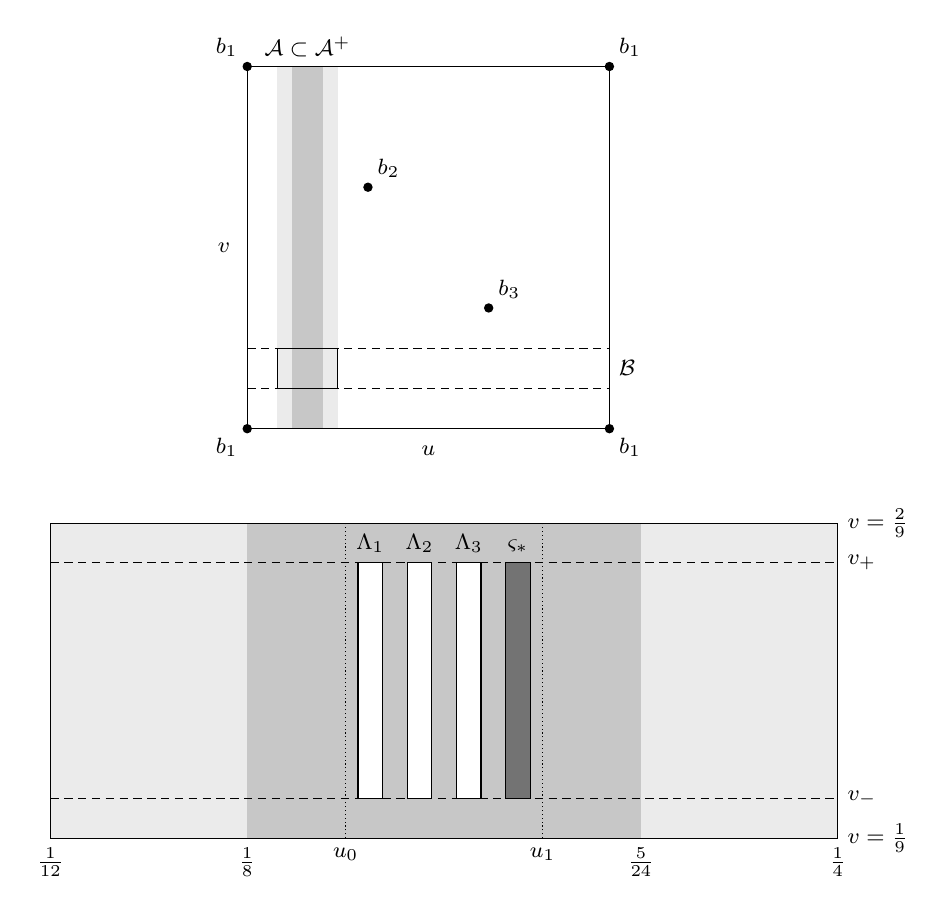
\begin{tikzpicture}[font=\footnotesize]
 \begin{scope}[scale=4.6]
  \fill[black!8] (1/12,0) rectangle (1/4,1);
  \fill[black!22] (1/8,0) rectangle (5/24,1);
  \draw[densely dashed] (0,1/9) -- (1,1/9);
  \draw[densely dashed] (0,2/9) -- (1,2/9);
  \draw (0,0) rectangle (1,1);
  \draw[thin] (1/12,1/9) rectangle (1/4,2/9);
  \foreach \p in {(0,0),(1,0),(0,1),(1,1),(1/3,2/3),(2/3,1/3)} \fill \p circle (0.013);
  \node[below left] at (0,0) {$b_1$};
  \node[below right] at (1,0) {$b_1$};
  \node[above left] at (0,1) {$b_1$};
  \node[above right] at (1,1) {$b_1$};
  \node[above right] at (1/3,2/3) {$b_2$};
  \node[above right] at (2/3,1/3) {$b_3$};
  \node[above] at (1/6,1) {$\mathcal A\subset\mathcal A^+$};
  \node[right] at (1,1/6) {$\mathcal B$};
  \node[below] at (1/2,-0.02) {$u$};
  \node[left] at (-0.02,1/2) {$v$};
 \end{scope}
 \begin{scope}[shift={(-2.5,-5.2)},x=60cm,y=36cm,shift={(-1/12,-1/9)}]
  \fill[black!8] (1/12,1/9) rectangle (1/4,2/9);
  \fill[black!22] (1/8,1/9) rectangle (5/24,2/9);
  \draw (1/12,1/9) rectangle (1/4,2/9);
  \draw[densely dashed] (1/12,1/8) -- (1/4,1/8);
  \draw[densely dashed] (1/12,5/24) -- (1/4,5/24);
  \filldraw[fill=white] (0.14844,1/8) rectangle (0.15365,5/24);
  \node[above] at (0.15104,5/24) {$\Lambda_1$};
  \filldraw[fill=white] (0.15885,1/8) rectangle (0.16406,5/24);
  \node[above] at (0.16146,5/24) {$\Lambda_2$};
  \filldraw[fill=white] (0.16927,1/8) rectangle (0.17448,5/24);
  \node[above] at (0.17188,5/24) {$\Lambda_3$};
  \filldraw[fill=black!55] (0.17969,1/8) rectangle (0.18490,5/24);
  \node[above] at (0.18229,5/24) {$\varsigma_*$};
  \draw[densely dotted] (7/48,1/9) -- (7/48,2/9);
  \draw[densely dotted] (3/16,1/9) -- (3/16,2/9);
  \node[below] at (7/48,1/9) {$u_0$};
  \node[below] at (3/16,1/9) {$u_1$};
  \node[below] at (1/8,1/9) {$\frac18$};
  \node[below] at (5/24,1/9) {$\frac5{24}$};
  \node[below] at (1/12,1/9) {$\frac1{12}$};
  \node[below] at (1/4,1/9) {$\frac14$};
  \node[right] at (1/4,1/8) {$v_-$};
  \node[right] at (1/4,5/24) {$v_+$};
  \node[right] at (1/4,1/9) {$v=\frac19$};
  \node[right] at (1/4,2/9) {$v=\frac29$};
 \end{scope}
\end{tikzpicture}
\caption{The handle data on the base torus $\Gamma=(\R/\Z)^2$ in the coordinates $(u,v)$ (Proposition~\ref{prop:cub-handle},
Definition~\ref{def:shd4-frame}). Top: the annuli $\mathcal A\subset\mathcal A^+$ (dark and light grey), the dual band
$\mathcal B$ (between the dashed lines $v=\frac19$, $v=\frac29$) and the marked points $b_1,b_2,b_3$, at which $Z_0=0$. Bottom: the rectangle
$\mathcal A^+\cap\mathcal B$ enlarged, with dashed lines at $v=v_\pm$; the clock $f$ rises on $[u_0,u_1]$, and the layers $\Lambda_i$ (white) and the
residual layer, where $\varsigma_*$ rises (black), lie over $(l_j,r_j)\times(v_-,v_+)$, where $b>0$. Drawn for $k=3$.}
\label{fig:shd4-handle}
\end{figure}

\begin{lemma}[The first path in the frame]\label{lem:shd4-frame-forms}
\lean{SymplecticPacking.Handle.Cubic.OmegaT_frameA, SymplecticPacking.Handle.Cubic.OmegaT_one_frameA,
SymplecticPacking.Handle.Cubic.Omega1Loc}
Over $\mathcal A^+$, $\chi_{\mathcal A}^*\Omega_t=\omega_V+\kappa_t+dp\wedge(a_{\mathcal A}+t\,\partial_p\alpha_1)$ with the positive forms
$\kappa_t$ of Lemma~\ref{lem:fer-positivity}. Over $\mathcal A$,
\[
 \chi_{\mathcal A}^*\Omega_1=\omega_V+e_h\nu+d\bigl(f(u)H^*(p)\beta\bigr).
\]
\end{lemma}

\begin{proof}
The first identity is Lemma~\ref{lem:fer-positivity}, written in the frame of Lemma~\ref{lem:fer-frame}. The second
is Lemma~\ref{lem:fer-alpha1}(ii), with $d\Gamma_{\rm sm}=e_h\nu$.
\end{proof}

\emph{The twist.} For $\lambda\in\R$ define on $\mathcal A\times\C$
\begin{equation}\label{eq:shd4-twist}
\begin{gathered}
 \mathcal D_\lambda(u,v,w_{\mathcal A})=\bigl(u,v,q_{\lambda f(u)}(w_{\mathcal A})\bigr),\qquad
 \mathcal D_\lambda^{-1}(u,v,w_{\mathcal A})=\bigl(u,v,q^{-1}_{\lambda f(u)}(w_{\mathcal A})\bigr),\\
 Q^\lambda_u=\lambda f'(u)\,Q_{\lambda f(u)},\qquad G_\lambda(u,w_{\mathcal A})=f(u)\,H^*\bigl(p(q_\lambda^{-1}w_{\mathcal A})\bigr),
\end{gathered}
\end{equation}
and $\mathcal D=\mathcal D_1$. These maps are smooth in $(\lambda,u,v,w_{\mathcal A})$ and mutually inverse, fix base points and
preserve $\mathcal A\times D(c)$ for every $c>P_{\rm supp}$.
\lean{SymplecticPacking.Handle.Cubic.Dlam, SymplecticPacking.Handle.Cubic.DlamInv, SymplecticPacking.Handle.Cubic.Qs,
SymplecticPacking.Handle.Cubic.Glam}

\begin{lemma}[Suspension]\label{lem:shd4-suspension}
\lean{SymplecticPacking.Handle.Cubic.suspension}
On $\mathcal A\times\C$, $\mathcal D_\lambda^*\omega_V=\omega_V+d\bigl[(Q^\lambda_u\circ q_{\lambda f(u)})\,du\bigr]$ for every $\lambda$.
\end{lemma}

\begin{proof}
This is \Mref{Lemma}{lem:hdl-suspension}(i) with $m=1$ and $s$ replaced by $u$: the differential of $\mathcal D_\lambda$ fixes
$\partial_v$, maps a vertical vector $\xi$ to $Dq\,\xi$ and $\partial_u$ to $\partial_u+X_{Q^\lambda_u}$, and $q_{\lambda f(u)}$ is symplectic.
\end{proof}

\emph{Periodisation.} For a one-form $\alpha$ on $\widetilde N$ supported over $\{u_0\le u\le u_1\}$ put
$\operatorname{per}(\alpha)=\sum_{m\in\Z}(T_u^m)^*\alpha$. The supports of the summands lie over the disjoint intervals
$[u_0-m,u_1-m]$, so the sum is locally finite; $\operatorname{per}(\alpha)$ is $T_u$-invariant, agrees with $\alpha$ over
$\{u_1-1<u<1+u_0\}$, and vanishes near every point whose $u$-coordinate is not in $[u_0,u_1]+\Z$. If $\alpha$ is horizontal, then
at a point with $\lfloor u\rfloor=m$ it is the covector of $\alpha$ at $T_u^{-m}$ of that point.
\lean{SymplecticPacking.Handle.Ush, SymplecticPacking.Handle.perJ}

\begin{construction}[The second-path primitive]\label{cons:shd4-eta}
\lean{SymplecticPacking.Handle.Cubic.etaLoc, SymplecticPacking.Handle.Cubic.eta, SymplecticPacking.Handle.Cubic.etaPer,
SymplecticPacking.Handle.Cubic.etaDot, SymplecticPacking.Handle.Cubic.OmS1}
On $\mathcal A\times\C$ let
\[
 \upsilon^{\mathcal A}_\lambda=\bigl(Q^\lambda_u\circ q_{\lambda f(u)}\bigr)\,du
 +f(u)\Bigl[H^*\bigl(p(q_\lambda^{-1}q_{\lambda f(u)}w_{\mathcal A})\bigr)-H^*\bigl(p(w_{\mathcal A})\bigr)\Bigr]\beta .
\]
Let $\upsilon_\lambda$ be the one-form on $\widetilde N$ equal to $(\chi_{\mathcal A}^{-1})^*\upsilon^{\mathcal A}_\lambda$ over $\mathcal A$ and to zero
elsewhere, let $\upsilon^{\rm per}_\lambda=\operatorname{per}(\upsilon_\lambda)$, and put
\[
 \Omega^{(1)}_\lambda=\Omega_1+d\upsilon^{\rm per}_\lambda,\qquad \dot\upsilon_\lambda=\partial_\lambda\upsilon^{\rm per}_\lambda .
\]
\end{construction}

\begin{lemma}[Properties of the second-path primitive]\label{lem:shd4-eta}
\lean{SymplecticPacking.Handle.Cubic.etaLoc_eq_zero_of_s, SymplecticPacking.Handle.Cubic.etaLoc_eq_zero_of_p,
SymplecticPacking.Handle.Cubic.eta_support, SymplecticPacking.Handle.Cubic.eta_smooth, SymplecticPacking.Handle.Cubic.eta_zero,
SymplecticPacking.Handle.Cubic.eta_horizontal, SymplecticPacking.Handle.Cubic.eta_TvE, SymplecticPacking.Handle.Cubic.etaDot_far,
SymplecticPacking.Handle.Cubic.firstStage_eq_pre}
\begin{enumerate}[label=(\alph*)]
\item $\upsilon^{\mathcal A}_\lambda$ vanishes for $u\le u_0$, for $u\ge u_1$, and for $p>P_{\rm supp}$; $\upsilon^{\mathcal A}_0=0$.
\item $\upsilon_\lambda$ and $\upsilon^{\rm per}_\lambda$ are horizontal one-forms on $\widetilde N$, smooth in $(\lambda,x)$; $\upsilon_\lambda$ is
$T_v$-invariant, $\upsilon^{\rm per}_\lambda$ is invariant under all deck maps, and $\upsilon^{\rm per}_0=0$. Both $\upsilon^{\rm per}_\lambda$ and $\dot\upsilon_\lambda$ vanish near every point with $p>P_{\rm supp}$ or with
$u\notin[u_0,u_1]+\Z$.
\item Over $\mathcal A$,
$\chi_{\mathcal A}^*\Omega^{(1)}_\lambda=\mathcal D_\lambda^*\bigl(\omega_V+e_h\nu+d(G_\lambda\beta)\bigr)$.
\end{enumerate}
\end{lemma}

\begin{proof}
(a) For $u\le u_0$, $f=f'=0$. For $u\ge u_1$, $f'=0$ and $q_\lambda^{-1}q_{\lambda f(u)}=q_\lambda^{-1}q_\lambda=\mathrm{id}$, so the bracket vanishes.
For $p>P_{\rm supp}$, $Q_t=0$ near $w_{\mathcal A}$ and all $q_t$, $q_t^{-1}$ fix $w_{\mathcal A}$. At $\lambda=0$ both terms vanish.

(b) By (a), $\upsilon^{\mathcal A}_\lambda$ vanishes over collars of both ends of $\mathcal A$, so the extension by zero is smooth. The form
$\upsilon^{\mathcal A}_\lambda$ has only $du$ and $dv$ components, and $\chi_{\mathcal A}$ preserves base points, so $\upsilon_\lambda$ is horizontal.
The coefficients of $\upsilon^{\mathcal A}_\lambda$ are $1$-periodic in $v$, since $b$ is periodic and $\mathcal D_\lambda$, $G_\lambda$ do not
depend on $v$; with $\chi_{\mathcal A}(u,v+1,\cdot)=T_v\chi_{\mathcal A}(u,v,\cdot)$ this gives $T_v^*\upsilon_\lambda=\upsilon_\lambda$. The
periodisation is $T_u$-invariant, and $T_v$-invariant because $T_u$ and $T_v$ commute. The support statement follows from (a)
and the properties of $\operatorname{per}$, and it passes to the $\lambda$-derivative.

(c) Over $\mathcal A$ the form $\upsilon^{\rm per}_\lambda$ is $\upsilon_\lambda$. The map $\mathcal D_\lambda$ fixes base points, so it preserves $\nu$ and
$\beta$ and $\mathcal D_\lambda^*(G_\lambda\beta)=(G_\lambda\circ\mathcal D_\lambda)\beta$ with
$G_\lambda\circ\mathcal D_\lambda=f(u)H^*(p(q_\lambda^{-1}q_{\lambda f(u)}w_{\mathcal A}))$. Add
Lemma~\ref{lem:shd4-suspension} to Lemma~\ref{lem:shd4-frame-forms}.
\end{proof}

\begin{proposition}[The second path]\label{prop:shd4-second}
\lean{SymplecticPacking.Handle.Cubic.OmegaPreG_split, SymplecticPacking.Handle.Cubic.firstStage_nondeg,
SymplecticPacking.Handle.Cubic.OmS1_preserves, SymplecticPacking.Handle.Cubic.twist_bound,
SymplecticPacking.Handle.Cubic.Hstar_twist_nonneg}
For valid cubic data and $\lambda\in[0,1]$, the form $\Omega^{(1)}_\lambda$ is closed, invariant under all deck maps, equal to
$\Omega_1$ for $\lambda=0$, and nondegenerate at every point of $\{p<h+2\delta_m\}$.
\end{proposition}

\begin{proof}
Closedness, invariance and $\Omega^{(1)}_0=\Omega_1$ follow from Lemma~\ref{lem:shd4-eta}(b) and the invariance of
$\Omega_1$ (Lemma~\ref{lem:fer-positivity}). Since deck maps preserve $p$ and the form, it suffices to check
nondegeneracy over $\{u_1-1<u<1+u_0\}$. Near points with $u\notin[u_0,u_1]$ the form is $\Omega_1$, which is symplectic
on $\{p<\frac13-e_h/9\}\supset\{p<h+2\delta_m\}$ (Lemmas~\ref{lem:fer-positivity} and~\ref{lem:shd4-budget}(d)). Over
$\mathcal A$ use Lemma~\ref{lem:shd4-eta}(c). By \Mref{Lemma}{lem:hdl-top-power}(b) with $n=2$, $\sigma_\Sigma=\nu$ and $e=e_h$,
\[
 \bigl(\omega_V+e_h\nu+d(G_\lambda\beta)\bigr)^2=2\bigl(e_h+b(v)\,\partial_uG_\lambda\bigr)\,\omega_V\wedge\nu,\qquad
 \partial_uG_\lambda(u,w')=f'(u)\,H^*\bigl(p(q_\lambda^{-1}w')\bigr).
\]
If $p(w_{\mathcal A})<h+2\delta_m$, then $w'=q_{\lambda f(u)}(w_{\mathcal A})$ and $q_\lambda^{-1}w'$ lie in $D(h+2\delta_m)$, because
$h+2\delta_m>P_{\rm supp}$; Lemma~\ref{lem:shd4-budget}(d) gives $H^*>0$ there. Since $f'\ge0$, $b\ge0$ and $e_h>0$, the
coefficient is positive at $\mathcal D_\lambda(x)$, and $\mathcal D_\lambda$ and $\chi_{\mathcal A}$ are diffeomorphisms.
\end{proof}

\emph{The final coefficient.} With the residual of Definition~\ref{def:shd4-scalars} put
\[
 G_{\rm f}(u,w)=J\bigl(p(w)\bigr)+\sum_{i=1}^k\varsigma_i(u)\,h_i\bigl(p(w)\bigr)+\varsigma_*(u)\,R^*(w),\qquad
 A_i=J+\sum_{j<i}h_j .
\]
\lean{SymplecticPacking.Handle.Cubic.Gf, SymplecticPacking.Handle.Cubic.aLayer}

\begin{lemma}[The final coefficient]\label{lem:shd4-Gf}
\lean{SymplecticPacking.Handle.Cubic.contDiff_Gf, SymplecticPacking.Handle.Cubic.Gf_mono, SymplecticPacking.Handle.Cubic.Gf_low,
SymplecticPacking.Handle.Cubic.Gf_up, SymplecticPacking.Handle.Cubic.Gf_layer}
For valid cubic data, $G_{\rm f}$ is smooth on $\R\times\C$ and
\begin{enumerate}[label=(\alph*)]
\item $\partial_uG_{\rm f}=\sum_i\varsigma_i'h_i\circ p+\varsigma_*'R^*\ge0$ at every $(u,w)$ with $R^*(w)\ge0$;
\item $G_{\rm f}=J\circ p$ for $u\le l_1$, and $G_{\rm f}=K\circ p\circ q^{-1}$ for $u\ge r_*$;
\item $G_{\rm f}(u,w)=A_i(p(w))+\varsigma_i(u)h_i(p(w))$ for $l_i<u<r_i$, $1\le i\le k$.
\end{enumerate}
\end{lemma}

\begin{proof}
(a) Differentiate; $h_i>0$ by Lemma~\ref{lem:shd4-budget}(a), and $\varsigma_j'\ge0$. (b) For $u\le l_1$ all clocks vanish. For
$u\ge r_*$ all equal one, and $J+\sum_ih_i+R^*=K\circ p\circ q^{-1}$. (c) On $(l_i,r_i)$, $\varsigma_j=1$ for $j<i$ and $\varsigma_j=0$ for
$j>i$, including $j=*$.
\end{proof}

\begin{construction}[The third-path primitive]\label{cons:shd4-xi}
\lean{SymplecticPacking.Handle.Cubic.Gdiff, SymplecticPacking.Handle.Cubic.xiA, SymplecticPacking.Handle.Cubic.JbE,
SymplecticPacking.Handle.Cubic.xi, SymplecticPacking.Handle.Cubic.xiPer, SymplecticPacking.Handle.Cubic.OmS2,
SymplecticPacking.Handle.Cubic.OmegaFinalPer, SymplecticPacking.Handle.Cubic.Ghat}
On $\mathcal A\times\C$ let $\xi^{\mathcal A}=\bigl((G_{\rm f}-G_1)\circ\mathcal D\bigr)\beta$. Let $\xi$ be the one-form on $\widetilde N$ equal to
$J(p)\beta+(\chi_{\mathcal A}^{-1})^*\bigl(\xi^{\mathcal A}-J(p)\beta\bigr)$ over $\mathcal A$ and to $J(p)\beta$ elsewhere, and put
\[
\begin{gathered}
 \xi^{\rm per}=J(p)\beta+\operatorname{per}\bigl(\xi-J(p)\beta\bigr),\qquad
 \Omega^{(2)}_\tau=\Omega^{(1)}_1+\tau\,d\xi^{\rm per},\\
 \Omega_{\rm fin}=\Omega^{(2)}_1,\qquad \hat G_\tau=(1-\tau)G_1+\tau G_{\rm f}.
\end{gathered}
\]
\end{construction}

\begin{lemma}[Properties of the third-path primitive]\label{lem:shd4-xi}
\lean{SymplecticPacking.Handle.Cubic.xi_collar, SymplecticPacking.Handle.Cubic.xi_smooth,
SymplecticPacking.Handle.Cubic.xi_horizontal, SymplecticPacking.Handle.Cubic.xi_toric_near_boundary,
SymplecticPacking.Handle.Cubic.xi_TvE, SymplecticPacking.Handle.Cubic.xiPer_deck, SymplecticPacking.Handle.Cubic.xiPer_eq_fX,
SymplecticPacking.Handle.Cubic.fX_far, SymplecticPacking.Handle.Cubic.secondStage_eq_on_A,
SymplecticPacking.Handle.Cubic.secondStage_off}
\begin{enumerate}[label=(\alph*)]
\item $\xi^{\mathcal A}=J(p)\beta$ for $u\le u_0$ and for $u\ge u_1$.
\item $\xi^{\rm per}$ is a smooth one-form on $\widetilde N$, invariant under all deck maps, of the form $\Xi\,\beta$ with $\Xi$ smooth; on
$\{p>P_{\rm supp}\}$, $\Xi$ is a function of $(u\bmod1,p)$.
\item Over $\mathcal A$, $\chi_{\mathcal A}^*\Omega^{(2)}_\tau=\mathcal D^*\bigl(\omega_V+e_h\nu+d(\hat G_\tau\beta)\bigr)$; near points with
$u\notin[u_0,u_1]+\Z$, $\Omega^{(2)}_\tau=\Omega_1+\tau J'(p)\,b(v)\,dp\wedge dv$.
\end{enumerate}
\end{lemma}

\begin{proof}
(a) For $u\le u_0$, $\mathcal D=\mathrm{id}$, $G_1=0$ and $G_{\rm f}=J\circ p$, since $u_0<l_1$. For $u\ge u_1>r_*$,
$G_1\circ\mathcal D=H^*(p(q^{-1}qw_{\mathcal A}))=H^*(p)$ and $G_{\rm f}\circ\mathcal D=K(p(q^{-1}qw_{\mathcal A}))=K(p)$, whose difference is $J(p)$.

(b) By (a), $\xi-J(p)\beta$ vanishes over collars of both ends of $\mathcal A$ and is supported over $[u_0,u_1]$, so $\xi$ and
the periodisation are smooth. Both summands are multiples of $\beta$: $\chi_{\mathcal A}$ preserves base points. Invariance
follows as in Lemma~\ref{lem:shd4-eta}(b), and $J(p)\beta$ is invariant because deck maps preserve $p$ and $v\bmod1$. On
$\{p>P_{\rm supp}\}$ all $q_t$ are the identity, $\mathcal D=\mathrm{id}$, and $G_1$, $G_{\rm f}$ are functions of $(u,p)$.

(c) Over $\mathcal A$, $\xi^{\rm per}=\xi$ and $\chi_{\mathcal A}^*\xi=\xi^{\mathcal A}=\mathcal D^*((G_{\rm f}-G_1)\beta)$; add
Lemma~\ref{lem:shd4-eta}(c) at $\lambda=1$. Near points with $u\notin[u_0,u_1]+\Z$, $\upsilon^{\rm per}_1=0$ and $\xi^{\rm per}=J(p)\beta$, and
$d(J(p)\beta)=J'(p)b(v)\,dp\wedge dv$.
\end{proof}

\begin{proposition}[The third path and the final form]\label{prop:shd4-third}
\lean{SymplecticPacking.Handle.Cubic.secondStage_nondeg, SymplecticPacking.Handle.Cubic.OmS2_preserves,
SymplecticPacking.Handle.Cubic.OmegaFinalPer_eq, SymplecticPacking.Handle.Cubic.OmegaFinal_eq_pullback,
SymplecticPacking.Strip.Cubic.DinvN, SymplecticPacking.Strip.Cubic.DinvN_pullback}
For valid cubic data and $\tau\in[0,1]$, $\Omega^{(2)}_\tau$ is closed, invariant under all deck maps and nondegenerate at every
point of $\{p<h+2\delta_m\}$. Over $\mathcal A$,
\[
 \chi_{\mathcal A}^*\Omega_{\rm fin}=\mathcal D^*\Omega_{\rm pre},\qquad
 (\chi_{\mathcal A}\circ\mathcal D^{-1})^*\Omega_{\rm fin}=\Omega_{\rm pre},\qquad
 \Omega_{\rm pre}=\omega_V+e_h\nu+d(G_{\rm f}\beta),
\]
and $\chi_{\mathcal A}\circ\mathcal D^{-1}$ maps $\mathcal A\times D(h)$ diffeomorphically onto $\mathcal A\times D(h)$.
\end{proposition}

\begin{proof}
Closedness and invariance follow from Proposition~\ref{prop:shd4-second} and Lemma~\ref{lem:shd4-xi}(b). As before it
suffices to work over $\{u_1-1<u<1+u_0\}$. Over $\mathcal A$, by Lemma~\ref{lem:shd4-xi}(c) and
\Mref{Lemma}{lem:hdl-top-power}(b), the square is $2(e_h+b\,\partial_u\hat G_\tau)\,\omega_V\wedge\nu$ at the image point
$\mathcal D(x)$, and $\partial_u\hat G_\tau=(1-\tau)\partial_uG_1+\tau\partial_uG_{\rm f}$. For $p(x)<h+2\delta_m$ the image fibre point $w'$ has
$p(w')<h+2\delta_m$; $\partial_uG_1(u,w')\ge0$ as in Proposition~\ref{prop:shd4-second}, and $\partial_uG_{\rm f}(u,w')\ge0$ by
Lemmas~\ref{lem:shd4-Gf}(a) and~\ref{lem:shd4-budget}(d). Near points with $u\notin[u_0,u_1]$, Lemma~\ref{lem:shd4-xi}(c) adds to
$\Omega_1$ a term $dp\wedge(\cdot)$ with a base one-form; in the local form of Lemma~\ref{lem:fer-positivity} it only changes the
mixed part, so the square is still $2\omega_V\wedge\kappa_1>0$ (Lemma~\ref{lem:pre-top-power}). The displayed identities are
Lemma~\ref{lem:shd4-xi}(c) at $\tau=1$. The last statement holds because $\mathcal D^{\pm1}$ fix base points and $q_t^{\pm1}$ preserve
$D(h)$, while $\chi_{\mathcal A}$ preserves $p$.
\end{proof}

\begin{lemma}[Vanishing on the marked fibres]\label{lem:shd4-fibres}
\lean{SymplecticPacking.Handle.fibreSetH, SymplecticPacking.Handle.Cubic.alpha1E_fibre,
SymplecticPacking.Handle.Cubic.etaDot_fibre, SymplecticPacking.Handle.Cubic.xiPer_fibre,
SymplecticPacking.Handle.Cubic.xi_zero_of_bB, SymplecticPacking.Handle.Cubic.xiPer_fibre}
Let $\widetilde{\mathcal F}$ be the union of all lifts of the fibres $N_{b_1},N_{b_2},N_{b_3}$, that is, the set of points
$(u,v,w)$ with $(u,v)\in b_j+\Z^2$ for some $j$. At every point of $\widetilde{\mathcal F}$ the covectors $\alpha_1$, $\dot\upsilon_\lambda$ $(\lambda\in\R)$ and $\xi^{\rm per}$ of
$T^*\widetilde N$ are zero.
\end{lemma}

\begin{proof}
For $\alpha_1$ this is Lemma~\ref{lem:fer-alpha1-fibres}, lifted to the cover, where $\alpha_1$ is periodic. The
$u$-coordinates of the $b_j$ are $0,\frac13,\frac23$, which are not in $[u_0,u_1]=[\frac7{48},\frac9{48}]$ modulo one, so
$\dot\upsilon_\lambda$ vanishes near $\widetilde{\mathcal F}$ by Lemma~\ref{lem:shd4-eta}(b). By Lemma~\ref{lem:shd4-xi}(b),
$\xi^{\rm per}=\Xi\,b(v)\,dv$; the $v$-coordinates of the $b_j$ are $0,\frac23,\frac13$, and $b$ vanishes outside
$[\frac18,\frac5{24}]+\Z$ (Proposition~\ref{prop:cub-handle}(c)), so $\beta$ vanishes at every point of
$\widetilde{\mathcal F}$.
\end{proof}

\begin{construction}[The handle Moser map]\label{cons:shd4-moser}
\lean{SymplecticPacking.Handle.Cubic.stage0, SymplecticPacking.Handle.Cubic.stage1, SymplecticPacking.Handle.Cubic.stage2,
SymplecticPacking.Handle.clock, SymplecticPacking.Handle.moserPathB, SymplecticPacking.Handle.moserVariationB,
SymplecticPacking.Handle.concat3B, SymplecticPacking.Handle.Cubic.handleData, SymplecticPacking.Handle.Cubic.handleParams,
SymplecticPacking.Handle.solve4, SymplecticPacking.Handle.cutoffChi, SymplecticPacking.Handle.boxFieldP,
SymplecticPacking.Handle.Cubic.handlePhi, SymplecticPacking.Handle.Cubic.handlePhiInv}
The three stages are
\[
 (\Omega^{(0)}_s,\mathfrak v^{(0)}_s)=(\Omega_s,\alpha_1),\qquad
 (\Omega^{(1)}_s,\mathfrak v^{(1)}_s)=(\Omega^{(1)}_s,\dot\upsilon_s),\qquad
 (\Omega^{(2)}_s,\mathfrak v^{(2)}_s)=(\Omega^{(2)}_s,\xi^{\rm per}),
\]
with matching endpoints $\Omega^{(0)}_1=\Omega^{(1)}_0$ and $\Omega^{(1)}_1=\Omega^{(2)}_0$. With the clocks $\sigma_i(t)=S(9t-3i-1)$,
$i=0,1,2$, which move only on $[\frac{3i+1}9,\frac{3i+2}9]$, put
\[
 \Omega^{\rm M}_t=\Omega^{(0)}_{\sigma_0(t)}+\sum_{i=1,2}\bigl(\Omega^{(i)}_{\sigma_i(t)}-\Omega^{(i)}_0\bigr),\qquad
 \mathfrak v_t=\sum_{i=0}^2\sigma_i'(t)\,\mathfrak v^{(i)}_{\sigma_i(t)} .
\]
On $U=\{p<h+2\delta_m\}$ let $Y_t$ be the field with $\iota_{Y_t}\Omega^{\rm M}_t=-\mathfrak v_t$; in the coordinates
$(\operatorname{Re}w,\operatorname{Im}w,u,v)$ it is the adjugate solution of a $4\times4$ skew system. With the moment cutoff
\[
 \mathfrak c(p)=S\Bigl(\frac{h+\frac74\delta_m-p}{\delta_m/4}\Bigr),
\]
which equals one for $p\le h+\frac32\delta_m$ and zero for $p\ge h+\frac74\delta_m$, let $\widehat Y_t=\mathfrak c(p)Y_t$, extended by zero.
The handle Moser map $\Phi$ is the time-one map of $\widehat Y$ from time $0$, and $\Phi^{-1}$ is its inverse.
\end{construction}

The bordered construction of \Msec{sec:hdl} cuts each path off by a whole-path Gram cutoff of a finite atlas,
because nondegeneracy is known only near the compact model region. Here the cover has one global chart and every stage
form is nondegenerate on the whole set $U$ for parameters in $[0,1]$; the moment cutoff $\mathfrak c(p)$ is the only cutoff, and
completeness comes from deck invariance.

\begin{proposition}[The handle Moser map]\label{prop:shd4-moser}
\lean[needed]{SymplecticPacking.Handle.Cubic.handleMoser, SymplecticPacking.Handle.handle_moser_global,
SymplecticPacking.Handle.Cubic.OmegaT_toric, SymplecticPacking.Handle.Cubic.etaDot_far,
SymplecticPacking.Handle.Cubic.d1_xiPer_toric, SymplecticPacking.Handle.Cubic.handleData_pres}
For valid cubic data, $\Phi$ and $\Phi^{-1}$ are mutually inverse $C^\infty$ diffeomorphisms of $\widetilde N$, and:
\begin{enumerate}[label=(\alph*)]
\item $\Phi^*\Omega_{\rm fin}=\Omega_0$ and $(\Phi^{-1})^*\Omega_0=\Omega_{\rm fin}$ at every point of $\{p\le h+\delta_m\}$;
\item for every $c>P_{\rm supp}$, $\Phi$ and $\Phi^{-1}$ map each of $\{p\le c\}$, $\{p<c\}$, $\{p=c\}$ onto itself;
\item $\Phi$ and $\Phi^{-1}$ fix every point of $\widetilde{\mathcal F}$;
\item $\Phi$ and $\Phi^{-1}$ commute with every deck map.
\end{enumerate}
Moreover $\Phi=\Phi_2\circ\Phi_1\circ\Phi_0$, where $\Phi_i$ is the time-one map of the cut stage field $\mathfrak c(p)Y^{(i)}_s$,
$\iota_{Y^{(i)}_s}\Omega^{(i)}_s=-\mathfrak v^{(i)}_s$.
\end{proposition}

\begin{proof}
\emph{Hypotheses.} On $[\frac{3i+1}9,\frac{3i+2}9]$ only $\sigma_i$ moves, so by the matching endpoints $\Omega^{\rm M}_t=\Omega^{(i)}_{\sigma_i(t)}$
there, and $\Omega^{\rm M}_t$ is $\Omega_0$ for $t\le\frac19$ and $\Omega_{\rm fin}$ for $t\ge\frac89$. Hence $\Omega^{\rm M}_t$ is closed and
nondegenerate on $U$ for every $t$ (Lemma~\ref{lem:fer-positivity} with Lemma~\ref{lem:shd4-budget}(d), and
Propositions~\ref{prop:shd4-second}, \ref{prop:shd4-third}). The pair is smooth on $\R\times\widetilde N$, and $\partial_t\Omega^{\rm M}_t=d\mathfrak v_t$ because
$\partial_s\Omega^{(i)}_s=d\mathfrak v^{(i)}_s$ for each stage; $\mathfrak v_t=0$ for $t\notin(0,1)$. By
Lemma~\ref{lem:pre-moser}(a), $Y$ is smooth on $\R\times U$, so $\widehat Y$ is smooth on $\R\times\widetilde N$. All stage forms and
primitives are deck invariant, and so is $\mathfrak c(p)$, since the deck maps preserve $p$.

\emph{Toric band.} Let $R=2\pi(-y\partial_x+x\partial_y)$, $w=x+iy$, generate the fibre rotation, so that $\iota_R\Omega_0=-dp$
(Lemma~\ref{lem:fer-positivity}). On $U'=\{P_{\rm supp}<p<h+2\delta_m\}$ one has $\iota_R\Omega^{\rm M}_t=-dp$ and $\mathfrak v_t(R)=0$:
$\alpha_1$ is horizontal and $\iota_Rd\alpha_1=0$; $\upsilon^{\rm per}_s$ and $\dot\upsilon_s$ vanish near $U'$
(Lemma~\ref{lem:shd4-eta}(b)); and on $U'$, $\xi^{\rm per}=\Xi(u\bmod1,p)\,b(v)\,dv$, whose differential has no fibre-angle
component, so $\iota_Rd\xi^{\rm per}=0=\xi^{\rm per}(R)$. Lemma~\ref{lem:pre-moser}(d) gives $dp(\widehat Y_t)=0$ on $\{p>P_{\rm supp}\}$, where
$\widehat Y$ vanishes for $p\ge h+\frac74\delta_m$.

\emph{Completeness.} The functions $du(\widehat Y_t)$, $dv(\widehat Y_t)$ are deck invariant (Lemma~\ref{lem:pre-moser}(g), since the
stage data and $\mathfrak c(p)$ are deck invariant), and deck maps
act on $(u,v)$ by integral translations; hence $|du(\widehat Y_t)|+|dv(\widehat Y_t)|\le C_b$, the maximum over the compact set
$[0,1]\times[0,1]^2\times\bar D(h+\frac74\delta_m)$, and $\widehat Y_t=0$ for $t\notin[0,1]$. By the toric band, an integral curve
through $x$ stays in $\{p\le\max(p(x),h)\}$, and its base coordinates move by at most $C_b$ in unit time. Integral curves
therefore remain in compact sets, and the flow and its inverse are defined on $\R\times\widetilde N$ and smooth.

\emph{Conclusions.} (b) follows from $dp(\widehat Y_t)=0$ on $\{p>P_{\rm supp}\}$, in both time directions. (a) For
$p(x)\le h+\delta_m$ the integral curve stays in $\{p\le h+\delta_m\}$, because $dp(\widehat Y_t)=0$ on $\{p>P_{\rm supp}\}$ (toric band)
and $P_{\rm supp}<h$. For the same reason the open set $\{p<h+\frac32\delta_m\}$ is invariant under the flow of $\widehat Y$, and
$\mathfrak c=1$ there, so $\widehat Y=Y$ on it and $\Phi$ agrees with the time-one map of the uncut field $Y$ on a neighbourhood of $x$.
Lemma~\ref{lem:pre-moser}(b) gives $(\Phi^*\Omega^{\rm M}_1)_x=(\Omega^{\rm M}_0)_x$. The inverse identity follows because
$\Phi^{-1}$ preserves $\{p\le h+\delta_m\}$. (c) By Lemma~\ref{lem:shd4-fibres}, $\mathfrak v_t=0$ on $\widetilde{\mathcal F}$ for every $t$,
so $\widehat Y_t=0$ there, and Lemma~\ref{lem:pre-moser}(c) applies in both time directions. (d) is
Lemma~\ref{lem:pre-moser}(g), since all stage forms and primitives and $\mathfrak c(p)$ are deck invariant.

\emph{Decomposition.} Each stage pair $(\Omega^{(i)}_s,\mathfrak v^{(i)}_s)$ is deck invariant and satisfies the same
rotation identity $\iota_R\Omega^{(i)}_s=-dp$, $\mathfrak v^{(i)}_s(R)=0$ on $U'$, so the completeness argument above applies
to each cut stage field $\mathfrak c(p)Y^{(i)}_s$; write $\Phi^{(i)}_s$ for its flow from time $0$ and $\Phi_i=\Phi^{(i)}_1$. On
$[\frac{3i+1}9,\frac{3i+2}9]$ the cut field is $\widehat Y_t=\sigma_i'(t)\mathfrak c(p)Y^{(i)}_{\sigma_i(t)}$, so
$t\mapsto\Phi^{(i)}_{\sigma_i(t)}(x)$ is an integral curve of $\widehat Y$ on that interval; on the gaps between these
intervals and for $t\notin[\frac19,\frac89]$ one has $\mathfrak v_t=0$, hence $\widehat Y_t=0$. By uniqueness of integral
curves, the integral curve of $\widehat Y$ through $x$ is obtained by running $\Phi^{(0)}$, $\Phi^{(1)}$, $\Phi^{(2)}$ in turn,
which gives $\Phi=\Phi_2\circ\Phi_1\circ\Phi_0$ (Lemma~\ref{lem:pre-moser}(f)).
\end{proof}

Equivalently, $\Phi$ is defined through compactly supported fields: for $A\ge0$ multiply $\widehat Y$ by a product
cutoff in $(u,v)$ equal to one on $\{|u|,|v|\le A+C_b+2\}$, let $\Phi_A$ be the time-one map of the cut field, and set $\Phi(x)=\Phi_A(x)$ with $A=|u(x)|+|v(x)|$. The base
speed bound shows that the integral curve through $x$ never meets the region where the box cutoff differs from one, so
this is the time-one map above.
\lean{SymplecticPacking.Handle.boxCut, SymplecticPacking.Handle.Cb, SymplecticPacking.Handle.boxL,
SymplecticPacking.Handle.PhiB, SymplecticPacking.Handle.PhiG, SymplecticPacking.Handle.PhiGInv,
SymplecticPacking.Handle.lfield_boxField, SymplecticPacking.Handle.LField.flowFrom_isSol, SymplecticPacking.Handle.flowFrom_box_eq}

\emph{Layer maps.} On the layer $\Lambda_i=\{l_i<u<r_i,\ \frac18<v<\frac5{24},\ p<h\}$ (frame coordinates) let
$T(v)=\int_{1/8}^vb$, a diffeomorphism of $(\frac18,\frac5{24})$ onto $(0,1)$ with $dT=\beta$ and inverse $v(T)$, and
\[
 \ell(T)=\frac{e_h}{b(v(T))},\qquad x_i(u,T,p)=(u-l_i)\,\ell(T)+\varsigma_i(u)\,h_i(p).
\]
Then $\partial_ux_i=\ell+\varsigma_i'h_i>0$, $x_i=0$ at $u=l_i$ and $x_i>h_i(p)$ at $u=r_i$, so for $0<x<h_i(p)$ and $0<T<1$ there is
a unique root $u=\sigma_i(x,T,p)\in(l_i,r_i)$. For $1\le i\le k$ put $\bar\rho_i=(\rho_i+a_i)/2$, $\delta_i=a_i-\bar\rho_i$,
$\hat\rho_i=\bar\rho_i+\delta_i/4$, and for $(z_{\rm b},z_{\rm f})\in\Bo(\hat\rho_i)\subset\C^2$ with $(x,T)=\Psi_{\delta_i}(z_{\rm b})$
(Proposition~\ref{prop:hdl-strip}) and $p=\pi|z_{\rm f}|^2$,
\[
 E_i(z_{\rm b},z_{\rm f})=\Bigl(\sigma_i(x,T,p),\ v(T),\ e^{-2\pi iTA_i'(p)}z_{\rm f}\Bigr),\qquad
 f^N_i=\Phi^{-1}\circ\chi_{\mathcal A}\circ\mathcal D^{-1}\circ E_i .
\]
\lean{SymplecticPacking.Strip.Cubic.ell, SymplecticPacking.Strip.Cubic.layerX, SymplecticPacking.Strip.Cubic.layerRoot,
SymplecticPacking.Strip.Cubic.shear, SymplecticPacking.Strip.Cubic.srcMap, SymplecticPacking.Strip.Cubic.layerMap,
SymplecticPacking.Strip.Cubic.layerMap_eq, SymplecticPacking.Strip.Cubic.fN}

\begin{proposition}[The four-dimensional embeddings into the cover]\label{prop:shd4-maps}
\lean[needed]{SymplecticPacking.Strip.Cubic.x_lt_hi, SymplecticPacking.Strip.Cubic.layer_form,
SymplecticPacking.Strip.Cubic.shear_pullback, SymplecticPacking.Strip.Cubic.layerMap_symplectic,
SymplecticPacking.Strip.Cubic.layerMap_mem_annulus, SymplecticPacking.Strip.Cubic.layerMap_injective,
SymplecticPacking.Strip.Cubic.layerMap_disjoint, SymplecticPacking.Strip.Cubic.layerMap_compact,
SymplecticPacking.Strip.Cubic.fN_mem, SymplecticPacking.Strip.Cubic.fN_smooth, SymplecticPacking.Strip.Cubic.fN_symplectic,
SymplecticPacking.Strip.Cubic.fN_eq_imp, SymplecticPacking.Strip.Cubic.fN_disjoint,
SymplecticPacking.Strip.Cubic.fN_avoid_fibres, SymplecticPacking.Strip.Cubic.fN_eq_imp,
SymplecticPacking.Embed.Cubic.fcap_eq_imp}
Let the cubic data be valid and $1\le i,j\le k$. Then $\rho_i<\bar\rho_i<\hat\rho_i<a_i$, and:
\begin{enumerate}[label=(\alph*)]
\item $f^N_i$ is defined and smooth on $\Bo(\hat\rho_i)$, with values in $\{p<h\}\setminus\widetilde{\mathcal F}$, and
$(f^N_i)^*\Omega_0=\omega_0$;
\item $f^N_i$ is injective, $f^N_i(\Bo(\hat\rho_i))\cap f^N_j(\Bo(\hat\rho_j))=\varnothing$ for $i\ne j$, and $f^N_i(B(\bar\rho_i))$ is compact;
\item if $f^N_i(X)=T\,f^N_j(X')$ for a deck map $T$, then $T=\mathrm{id}$, $i=j$ and $X=X'$.
\end{enumerate}
\end{proposition}

\begin{proof}
Let $\varpi=\pi|z_{\rm b}|^2$ and $\varpi+p<\hat\rho_i$. By Proposition~\ref{prop:hdl-strip} and Lemma~\ref{lem:shd4-budget}(a),
\[
 0<x<\varpi+\frac{\delta_i}2<\hat\rho_i-p+\frac{\delta_i}2=a_i-p-\frac{\delta_i}4<h_i(p),\qquad p<a_i<h,
\]
so the root exists, and $E_i$ maps $\Bo(\hat\rho_i)$ into $\Lambda_i$. Since $\ell\,b=e_h$, $e_h\nu=\ell\,du\wedge dT$; with
Lemma~\ref{lem:shd4-Gf}(c), $d(G_{\rm f}\beta)=(\varsigma_i'h_i\,du+dA_i+\varsigma_i\,dh_i)\wedge dT$ on $\Lambda_i$, hence
$\Omega_{\rm pre}=\omega_V+dx_i\wedge dT+dA_i(p)\wedge dT$ there. $E_i$ is the composite
of $\Psi_{\delta_i}\times\mathrm{id}$, the shear of Lemma~\ref{lem:hdl-shear} with $A=A_i$ and the inverse of the layer coordinates
$(u,v,w_{\mathcal A})\mapsto(x_i,T,w_{\mathcal A})$ (the periodic counterpart of the layer maps of Proposition~\ref{prop:str-layer}); by Proposition~\ref{prop:hdl-strip} and Lemma~\ref{lem:hdl-shear} it is a diffeomorphism onto an open subset of $\Lambda_i$ with $E_i^*\Omega_{\rm pre}=\omega_0$.

(a) By Proposition~\ref{prop:shd4-third}, $\chi_{\mathcal A}\mathcal D^{-1}$ maps $\Lambda_i$ into $\mathcal A\times D(h)$ and pulls $\Omega_{\rm fin}$ back
to $\Omega_{\rm pre}$; by Proposition~\ref{prop:shd4-moser}(a),(b), $\Phi^{-1}$ preserves $\{p<h\}$ and pulls $\Omega_0$ back to
$\Omega_{\rm fin}$ there. Composing gives $(f^N_i)^*\Omega_0=\omega_0$. The point $\chi_{\mathcal A}\mathcal D^{-1}E_i(X)$ lies over $\mathcal A$,
which misses $\widetilde{\mathcal F}$; if $\Phi^{-1}(y)\in\widetilde{\mathcal F}$, then $y=\Phi(\Phi^{-1}y)=\Phi^{-1}y\in\widetilde{\mathcal F}$ by
Proposition~\ref{prop:shd4-moser}(c).

(b) $E_i$ is injective, the images of different $E_i$ lie over the disjoint intervals $(l_i,r_i)$, and
$\chi_{\mathcal A}\mathcal D^{-1}$ and $\Phi^{-1}$ are injective maps common to all $i$. The closed ball is compact.

(c) By Proposition~\ref{prop:shd4-moser}(d), $\Phi^{-1}(y)=T\Phi^{-1}(y')=\Phi^{-1}(Ty')$ with $y=\chi_{\mathcal A}\mathcal D^{-1}E_i(X)$ and
$y'=\chi_{\mathcal A}\mathcal D^{-1}E_j(X')$, so $y=Ty'$. Both points lie over the square $(\frac18,\frac5{24})^2$, so the shift of $T$ is
zero and $T=\mathrm{id}$; then (b) gives $i=j$ and $X=X'$.
\end{proof}

\begin{remark}[The four-dimensional embeddings]\label{rem:shd-four}
\lean{SymplecticPacking.Embed.Cubic.fcap, SymplecticPacking.Embed.Cubic.fcapV, SymplecticPacking.Branch2.CubicData.fcapGen,
SymplecticPacking.Handle.Cubic.handleMoser, SymplecticPacking.Strip.fN, SymplecticPacking.Embed.Cubic.fcap,
SymplecticPacking.Branch2.embeddings2, SymplecticPacking.Branch2.embeddingsEq, SymplecticPacking.Branch2.CubicData.ofParams}
By Proposition~\ref{prop:shd4-maps}(a),(c) the maps $f^N_i$ satisfy the hypotheses of Theorem~\ref{thm:cub-transfer}, and
the four-dimensional embeddings are
$f^{\rm cap}_i=b_{\rm ball}\circ\mathcal T_{\rm u}\circ\mathsf N\circ f^N_i$ on $\Bo(\hat\rho_i)$. The general branch uses the data of Proposition~\ref{prop:scalar-cubic-data}
and the capacities of \eqref{eq:scalar-enlargement}. The equal branch uses the same maps for the data of
Remark~\ref{rem:rtc-equal}: $\rho_i=\rho$, $a_i=a$, $K(p)=(3\sqrt k-9)p$, and $(q_t)$ the isotopy of
Theorem~\ref{thm:pll-inner}, with the recorded capacities of Remark~\ref{rem:rtc-recorded}. The strip constants are
the four-dimensional values recorded in Definition~\ref{def:str-enlarged}: $\delta_i=a_i-\bar\rho_i=(a_i-\rho_i)/2$ and
$\hat\rho_i=a_i-\frac34\delta_i$; only the disc-to-strip map of Proposition~\ref{prop:str-strip} is taken from \S\ref{sec:str},
and the layer identities are proved in Proposition~\ref{prop:shd4-maps}.
\end{remark}

\subsection{The shear and the strip map}\label{sec:shd-shear}

The two explicit maps used in the layers of \Msec{sec:hdl-layers} are the following.

\begin{lemma}[Multi-angle shear]\label{lem:hdl-shear}
\lean{OAI.PackingSufficiencySupport.Hamiltonian.toricSuspension,
OAI.PackingSufficiencySupport.Hamiltonian.toricSuspensionInverse_smooth,
OAI.PackingSufficiencySupport.Hamiltonian.toricSuspension_pullback,
OAI.PackingSufficiencySupport.Hamiltonian.toricSuspensionInverse_left,
OAI.PackingSufficiencySupport.Hamiltonian.toricSuspensionInverse_right}
\uses{M-def:mech-model}
Let $A$ be a smooth function on an open set $W\subset\R^m$ and $\mathrm{Sh}_A(x,T,w)=(x,T,\mathrm{Sh}_{A,T}(w))$, where
\[
 \mathrm{Sh}_{A,T}(w)_j=\exp\big(-2\pi i\,T\,\partial_jA(p(w))\big)\,w_j\qquad(1\le j\le m),
\]
on $\{(x,T,w):p(w)\in W\}\subset\R^2\times\C^m$. Then $\mathrm{Sh}_A$ is a diffeomorphism of this set onto itself, preserves
$p$, $x$ and $T$, and
\[
 \mathrm{Sh}_A^*\big(\omega_V+dx\wedge dT+dA(p)\wedge dT\big)=\omega_V+dx\wedge dT .
\]
\end{lemma}

\begin{proof}
$\mathrm{Sh}_{A,T}$ multiplies each $w_j$ by a unimodular factor that is a smooth function of $(T,p(w))$; it preserves $p$, and the
same formula with $+2\pi i$ is its inverse. Both are smooth in Cartesian coordinates, also on the coordinate axes. Where all
$w_j\ne0$, write $w_j=\sqrt{p_j/\pi}\,e^{2\pi i\theta_j}$, so $\mathrm{Sh}_{A,T}$ is $\theta_j\mapsto\theta_j-T\partial_jA(p)$. Then
\[
 \mathrm{Sh}_A^*\omega_V=\sum_jdp_j\wedge d\big(\theta_j-T\partial_jA\big)
 =\omega_V-dA\wedge dT-T\sum_{j,k}\partial_{jk}A\,dp_j\wedge dp_k=\omega_V-dA\wedge dT,
\]
the Hessian term vanishing by symmetry; $dx\wedge dT$ and $dA(p)\wedge dT$ are unchanged since $x,T,p$ are. The identity extends
to the coordinate axes by continuity.
\end{proof}

\begin{proposition}[Disc-to-strip map]\label{prop:hdl-strip}
\lean{SymplecticPacking.Strip.psiStrip, SymplecticPacking.Strip.psiStrip_smooth,
 SymplecticPacking.Strip.psiStrip_symplectic, SymplecticPacking.Strip.psiStrip_bijOn,
 SymplecticPacking.Strip.psiStrip_x_pos, SymplecticPacking.Strip.psiStrip_x_lt}
\uses{prop:str-strip}
For every $\delta>0$ there is an explicit smooth diffeomorphism
$\Psi_\delta\colon\C\to(0,\infty)\times(0,1)$, $z\mapsto(x,T)$, with $\Psi_\delta^*(dx\wedge dT)=\omega_\C$ and
\[
 0<x<\pi|z|^2+\frac\delta2\qquad\text{for all }z\in\C .
\]
\end{proposition}

The map is $\Psi_\delta=F\circ\mathsf T^{-1}\circ\mathsf D$, where $F(u,v)=(X(u),Y(v))$ inverts the square roots of the Morse
functions $x+\varepsilon^2/(4x)-\varepsilon$ on $(0,\infty)$ and $\varepsilon\,[(2\sqrt{T(1-T)})^{-1}-1]$ on $(0,1)$,
$\varepsilon=\delta/\pi$, and $\mathsf T,\mathsf D$ are the explicit rotation and radial area normalisations of the density
$X'(u)Y'(v)$. The estimate holds because the level set of energy $\mathcal E$ encloses area at least
$\mathcal E-\varepsilon(\frac\pi2-1)$ and lies in $\{x<\mathcal E+\varepsilon\}$ (Proposition~\ref{prop:str-strip}). A compact subset of
an open set of area $a$ has area less than $a$, so no area-preserving map takes the closed disc of area $a$ into
$\{0<x<a\}\times(0,1)$; the excess $\delta/2$ is paid once, for all concentric discs simultaneously.

